\documentclass[13pt]{beamer}
%%%%%%%% tema e cor %%%%%%%%
\mode<presentation> {
\usetheme{Madrid}
%\usecolortheme{albatross}
}

\usepackage[brazil]{babel}
\usepackage[utf8x]{inputenc}
\usepackage{graphicx} 
\usepackage{booktabs} 
\usepackage{pgfcore}
\usepackage{xxcolor}

\institute[UPE] 
{
%================= logos no meio =====================
\vspace*{-0.35cm}

\includegraphics[width=100px]{img/upe.jpeg}
\hspace*{0.25cm}~%

\includegraphics[width=100px]{img/fcm.jpeg}
\vspace*{0.35cm}\\
}
\date{19 de Agosto de 2019}

\AtBeginSection[]
{
\begin{frame}
\frametitle{Sumário}
\tableofcontents[currentsection]
\end{frame}
}
\title[Apresentação de DC]{Abdome agudo} 
\author[FCM]{Filipe Mosca, Gabriel Lucas, Johnny Folle \\
Prof. Bernardo Sabat} 

\begin{document}

\begin{frame}
\titlepage 

\end{frame}

\begin{frame}
\frametitle{Sumário} 
\tableofcontents 
\end{frame}

%%%%%%%% slides %%%%%%%%
\section{Identificação} 
\begin{frame}{Identificação}
\begin{itemize}
\item Nome: SVFSL
\item Sexo: Feminino
\item Idade: 20 anos
\item Procedência: Jaboatão dos Guararapes
\item Naturalidade: Camaragibe
\item Profissão: Estudante
\item Estado civil: Solteira
\end{itemize}
\end{frame}


\section{Queixa principal}
\begin{frame}{Queixa principal}
\begin{block}{}
Dor abdominal há 4 dias acompanhada de distensão
\end{block}
\end{frame}

\section{História da doença atual}
\begin{frame}{História da doença atual}
Mulher de 24 anos de idade, primigesta, nulípara, com 24 semanas de gestação, G0P1A0, procurou o serviço de emergência do Hospital da Restauração apresentando sintoma principal de dor abdominal nos últimos 4 dias acompanhada de distensão. A dor era insidiosa no início, de caráter agudo, localizada no quadrante inferior direito, mas aumentou progressivamente até envolver todo o abdome. O quadro estava associado a náuseas e vômitos. Além disso, a paciente refere não defecar nos últimos dois dias e dificuldade para urinar. 
\end{frame}

\begin{frame}{História da doença atual}
    \begin{itemize}
        \item Há 4 dias:
             \begin{itemize}
                 \item Apresentou sintoma principal de dor abdominal  insidiosa, de caráter agudo, localizada no quadrante inferior direito.
             \end{itemize}
        \item Associada à:
            \begin{itemize} 
                \item Distensão, náuseas, vômitos e febre.
            \end{itemize}
        \item Melhorava com:
            \begin{itemize} 
                \item Sem fatores de melhora.
            \end{itemize}
        \item Há 2 dias:
             \begin{itemize}
                 \item A dor evoluiu para difusa em todo abdome. 
             \end{itemize}
       \item Associada à:
         \begin{itemize}
             \item Ausência de movimentos intestinais.  
         \end{itemize}
    \end{itemize}
\end{frame}

\section{Interrogatório sintomatológico}
\begin{frame}{Interrogatório sintomatológico}
\begin{itemize}
    \item Geral: edema +1/+4 em MMII
    \item SNC/ORL: sem queixas
    \item Respiratório: dispneia leve;
    \item Cardiovascular: sem queixas
    \item Uroexcretor: incontinência urinária;
    \item Gastrointestinal: constipação, náuseas e vômitos, distensão, dor;
\end{itemize}{}
\end{frame}

\section{Antecedentes pessoais}
\begin{frame}{Antecedentes pessoais}
\begin{enumerate}
    \item Nega acometimento gastrointestinal anterior;
    \item Nega ter feito cirurgias;
    \item Refere ter vacinação em dia; 
    \item Nega ingesta de bebidas alcoólicas e nega tabagismo; 
    \item História de infecção urinária tratada há 2 anos.
\end{enumerate}{}
\end{frame}

\section{Antecedentes familiares}
\begin{frame}{Antecedentes familiares}
    \begin{itemize}
        \item Nega histórico de comorbidades gastrointestinais e doenças crônicas na família.
    \end{itemize}
\end{frame}


\section{Exame físico}
\begin{frame}{Exame físico}
    \begin{block}{Geral}
        \begin{itemize}
            \item Geral: EGR, consciente, orientada, hipocorada, anictérica, acianótica, febril ao toque;
            \item Peso: 70 Kg
            \item Altura: 1,63 cm
            \item Temperatura axilar: 38,6°C;
            \item FC: 104 bpm;
            \item FR: 24 ipm;
            \item PA: 110/76 mmHg.
        \end{itemize}{}
    \end{block}
\end{frame}

\begin{frame}{Exame físico}
    \begin{block}{Abdominal}
        \begin{itemize}
            \item Inspeção: abdome gravídico;
            \item Palpação: abdome tenso e distendido com sinais de defesa abdominal voluntária no quadrante inferior esquerdo; Fundo uterino palpável 3 cm acima da cicatriz umbilical e compatível com 24 semanas de gestação.
            \item Ausculta: RHA ausentes em todo o abdome.
        \end{itemize}{}
    \end{block}
    \begin{block}{Cardiovascular}
    Ausculta: RCR, 2T, BNF S/S
    \end{block}
    \begin{block}{Respiratório}
    Ausculta: MV+ em AHT, sem RA
    \end{block}
\end{frame}

\begin{frame}{Exame físico}
    \begin{block}{Genital}
        \begin{itemize}
            \item Toque vaginal: sem dor à mobilização do colo;
            \item Toque retal sem alterações.
        \end{itemize}{}
    \end{block}
\end{frame}

\section{Discussão}
\begin{frame}{Discussão}
\begin{block}{Problemas relevantes}
    \begin{itemize}
        \item Dor inicial em QID
        \item Abdome tenso
        \item Episódios eméticos
        \item Constipação intestinal
        \item Incontinência urinária
    \end{itemize}{}
\end{block}
\end{frame}

\begin{frame}{Discussão}
\begin{block}{Hipóteses diagnósticas}
    \pause
    \begin{itemize}
        \item Apendicite \pause
        \item Gravidez ectópica \pause
        \item Doença inflamatória pélvica \pause
        \item Litíase renal \pause
        \item Diverticulite de Meckel
    \end{itemize}{}
\end{block}
\end{frame}


\begin{frame}{Apendicite}
        \setbeamercolor{block title}{use=structure,fg=white,bg=green!75!black}
    \begin{columns}
    \column{0.5\textwidth}
        \begin{block}{A favor}
            \begin{itemize}
            \item Vômitos
            \item Dor em QID
            \item Febre
            \item Taquicardia
            \item Defesa abdominal
            \end{itemize}
        \end{block}
    \end{columns}
\end{frame}


\begin{frame}{Gravidez ectópica}
        \setbeamercolor{block title}{use=structure,fg=white,bg=green!75!black}
    \begin{columns}
    \column{0.4\textwidth}
        \begin{block}{A favor}
            \begin{itemize}
            \item Dor em QID intensa, aguda;
            \item Abdome doloroso a palpação;
            \item Náuseas e vômitos.
            \end{itemize}
        \end{block}
     
     \column{0.4\textwidth}
         \setbeamercolor{block title}{use=structure,fg=white,bg=red!75!black}
        \begin{block}{Contra}
            \begin{itemize}
             \item Sem dor a mobilização do colo uterino;
            \item Sem sangramento vaginal;
            \item Sem alterações hemodinâmicas graves (hemorragia);
            \item Sem abaulamento no fundo de saco;
            \item Febre.
            \end{itemize}
        \end{block}
    \end{columns}
\end{frame}

\begin{frame}{Doença inflamatória pélvica}
        \setbeamercolor{block title}{use=structure,fg=white,bg=green!75!black}
            \begin{columns}
            \column{0.5\textwidth}
                \begin{block}{A favor}
                    \begin{itemize}
                    \item Dor em QID
                    \item Náuseas e vômitos
                    \item Febre
                    \end{itemize}
                \end{block}
     
         \setbeamercolor{block title}{use=structure,fg=white,bg=red!75!black}
        \begin{block}{Contra}
            \begin{itemize}
                \item Gravidez\cite{abdou_postpartum_2017}
                \item Ausência de dor à mobilização uterina
            \end{itemize}
        \end{block}
    \end{columns}
\end{frame}

\begin{frame}{Litíase renal}
        \setbeamercolor{block title}{use=structure,fg=white,bg=green!75!black}
    \begin{columns}
    \column{0.5\textwidth}
        \begin{block}{A favor}
            \begin{itemize}
            \item Dor em QID, aguda, forte intensidade;
            \item Náuseas e vômitos;
            \item Febre (infecção urinária);
            \item Irritação peritoneal;
            \end{itemize}
        \end{block}
     
         \setbeamercolor{block title}{use=structure,fg=white,bg=red!75!black}
        \begin{block}{Contra}
            \begin{itemize}
             \item Sem disúria, polaciúria, hematúria;
            \item Sinal de Giordano negativo;
            \item Sem episódios anteriores de dor;
            \end{itemize}
        \end{block}
    \end{columns}
\end{frame}


\begin{frame}{Diverticulite de Meckel}
        \setbeamercolor{block title}{use=structure,fg=white,bg=green!75!black}
    \begin{columns}
    \column{0.5\textwidth}
        \begin{block}{A favor}
            \begin{itemize}
                \item Dor em QID, crescente
                \item Vômitos e náusea
            \end{itemize}
        \end{block}
     
        \setbeamercolor{block title}{use=structure,fg=white,bg=red!75!black}
        \begin{block}{Contra}
            \begin{itemize}
                \item Sem sangramento retal.
            \end{itemize}
        \end{block}
    \end{columns}
\end{frame}


\begin{frame}{Dificuldades do diagnóstico}
Na gestação, sintomas como náuseas e vômitos, desconforto abdominal e pélvico, são comuns e podem mascarar e confundir os sinais de uma afecção abdominal.\vspace{5mm} 

Além disso, a presença do útero ocupando grande parte da cavidade abdominal dificulta o exame físico.\vspace{5mm}

Leucocitose, anemia devido a hemodiluição e taquicardia são achados comuns em gestantes.
\end{frame}



\section{Exames complementares}
\begin{frame}{Exames complementares}
    \begin{block}{Leucograma}
    Leucopenia: 3.9×10\textsuperscript{3}/mm\textsuperscript{3} (VR = 5.6 a 14.8×10\textsuperscript{3}/mm\textsuperscript{3})\\
    Neutrofilia: 75\%
    \end{block}

    \begin{block}{USG}
    Revelou fluido livre na cavidade abdominal com múltiplas septações. Idetificada gestação única e tópica com feto saudável e diâmetros biparietais e femurais compatíveis com 24 semanas.
    \end{block}
    
    \begin{block}{Tomografia computadorizada}
    Não realizada com intutito de evitar exposição fetal.
    \end{block}
\end{frame}

\section{Diagnóstico e tratamento}
\begin{frame}{Diagnóstico e Tratamento}
    \begin{block}{}
    A paciente foi submetida a uma laparotomia exploradora. 
    \end{block}
    \vspace{5mm} 
    Foi evidenciado 1.5 L de secreção mucopurulenta na cavidade abdominal.\vspace{5mm}
    E encontrando um divertículo de Meckel perfurado de aproximadamente 2-3 cm de comprimento, localizado a 70 cm da junção íleo-cecal, na borda antimesentérica.
\end{frame}

\begin{frame}{Diagnóstico e Tratamento}
    \begin{figure}
        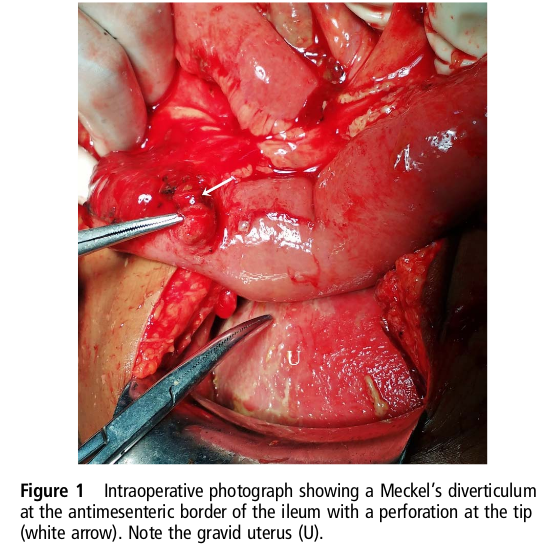
\includegraphics[width=220px]{img/foto.png}
    \end{figure}
\end{frame}


\begin{frame}{Diverticulo de Meckel}
    O divertículo de Meckel é a anomalia congênia do trato gastrointestial mais comum. Presente em 2 a 4\% da população.\vspace{5mm}
    
    As complicações mais comums são:
        \begin{itemize}
            \item Obstrução - 36,5\%
            \item Intussuscepção - 13,7\%
            \item Inflamação ou diverticulite - 12,7\%
            \item Hemorragia - 11,8\%
            \item Neoplasia - 3,2\%
            \item Fístula - 1,7\%
        \end{itemize}
\end{frame}

\begin{frame}{Diverticulo de Meckel}
    O tratamento do divertículo de Meckel em gestantes é o mesmo para pacientes não gestantes. \vspace{5mm}
    
    Consiste na cirurgia de diverticulotomia ou ressecção segmental seguida de anastomose.\vspace{5mm}
    
    Em casos de abdome séptico, a ileostomia é uma boa alternativa.
\end{frame}

%------------------------------------------------


%------------------------------------------------
%%%%%%%% referencias %%%%%%%%
\nocite{*}
\begin{frame}{Referências}
\bibliographystyle{unsrt}
\bibliography{ref.bib}
\end{frame}


%%%%%%%% repete primeiro slide %%%%%%%%
\begin{frame}
\titlepage 
\end{frame}
\end{document}